\documentclass{beamer}

\usepackage[utf8]{inputenc}
\usepackage[T2A]{fontenc}
\usepackage[russian]{babel}
\usepackage{url}

\usepackage{amsmath}
\usepackage{tikz}
\usepackage{graphicx}

\usetheme{Madrid}

\title{Исследование границ применимости процедурного кластерного видозависимого лоддирования в современных компьютерных играх}
\author{Антон Суркис}

\begin{document}
    \maketitle

    \begin{frame}{Введение}
        \begin{itemize}
            \item
            В современных компьютерных играх для реалистичной графики
            используют высокодетализированные модели объектов;

            \item
            Отрисовывать такие высокодетализированные модели для
            всех объектов на экране очень долго,
            а компьютерная игра должна реагировать на ввод
            в реальном времени;

            \item
            Стандартное решение --- рисовать объекты
            далеко от камеры в меньшем разрешении;

            \item
            Стандартное решение плохо работает для
            больших объектов, например, статуй и зданий,
            у которых одна часть может оказаться близко
            к камере, а другая --- далеко.
        \end{itemize}
    \end{frame}

    \begin{frame}{Введение}
        \begin{itemize}
            \item В 2020 году компания Epic Games представила
            существенно другой подход к оптимизации
            отрисовки высокодетализированных объектов
            --- технологию Nanite в движке Unreal Engine 5;

            \item Nanite из исходной геометрии объекта
            составляет набор стыкующихся между собой объектов,
            которые можно рисовать независимо
            друг от друга без заметных искажений;

            \item Так Nanite отрисовывает в высоком разрешении
            ту \emph{часть} большого объекта, которая близко к камере,
            и в низком --- ту, которая далеко.
        \end{itemize}
    \end{frame}

    \begin{frame}{Проблема}
        \begin{itemize}
            \item Несмотря на то,
            что Nanite представили ещё в 2020,
            а описание его работы открыто,
            далеко не все движки внедрили подобные технологии;

            \item Следовательно, у технологии есть
            какие-то значительные недостатки,
            сравнимые с преимуществами.
        \end{itemize}
    \end{frame}

    \begin{frame}{Цели и задачи}
        \textbf{Цель работы:}
        исследовать ограничения динамической кластерной детализации,
        существенные для компании-разработчика игр.

        \bigskip

        \textbf{Задачи:}
        \begin{itemize}
            \item Изучить механизм работы Nanite;
            \item Реализовать упрощённую систему
            динамической кластерной детализации;
            \item Определить проблемы, возникающие при реализации;
            \item Определить принципиальные ограничения технологии;
            \item Сравнить с ,,монолитной`` детализацией.
        \end{itemize}
    \end{frame}

    \begin{frame}{Nanite}
        Общий механизм работы
        Nanite\footnote{
            \url{https://advances.realtimerendering.com/s2021/Karis_Nanite_SIGGRAPH_Advances_2021_final.pdf}
        } состоит из двух этапов ---
        преобразование исходной модели и её отрисовка.

        Преобразование исходной модели:
        \begin{enumerate}
            \item Разбить треугольники модели объекта на кластеры, такие кластеры называются ,,мешлетами`` (meshlet);
            \item Скопировать полученные мешлеты как новые вершины графа;
            \item Объединить соседние мешлеты в кластеры по 4 \label{nanite-partition-begin};
            \item Уменьшить детализацию мешлета-кластера;
            \item Разбить кластер на 2 новых мешлета;
            \item Назначить оба новых мешлета ,,родителями`` тех, из которых составлен кластер \label{nanite-partition-end};
            \item Повторять шаги \ref{nanite-partition-begin}-\ref{nanite-partition-end},
            пока не останется мало (в идеале --- только 2) мешлетов без родителей.
        \end{enumerate}
    \end{frame}

    \begin{frame}{Nanite}
        Отрисовка полученного направленного ациклического графа:
        \begin{itemize}
            \item Каждый мешлет обрабатывается на видеокарте
            независимо от остальных;
            \item Новые видеокарты поддерживают отрисовку
            массивов мешлетов наравне с массивами треугольников;
            \item Отрисовываем мешлет только если оцениваем,
            что он достаточно близко к камере, чтобы
            отрисовка его родителей уже приводила к искажениям;
            \item Поэтому оценка ошибки должна монотонно
            убывать по мере спуска по графу;
            \item В результате высокой детализации исходной модели
            значительная часть треугольников мешлета будет
            иметь размер в 1 пиксель.
            Аппаратные оптимизации видеокарт сильно завязаны
            на то, что треугольники сильно больше 1 пикселя,
            поэтому маленькие треугольники в Nanite
            отрисовываются с помощью вычислительного шейдера.
        \end{itemize}
    \end{frame}

    \begin{frame}{Nanite, визуализация графа}
        Граф не является деревом,
        чтобы не возникало длинных несокращаемых швов:
        \begin{center}
            \begin{tikzpicture}
                \node[draw,circle] (n11) at (0,6) {};
                \node[draw,circle] (n12) at (1,6) {};
                \node[draw,circle] (n21) at (-1,4) {};
                \node[draw,circle] (n22) at (0,4) {};
                \node[draw,circle] (n23) at (1,4) {};
                \node[draw,circle] (n24) at (2,4) {};
                \node[draw,circle] (n31) at (-3,2) {};
                \node[draw,circle] (n32) at (-2,2) {};
                \node[draw,circle] (n33) at (-1,2) {};
                \node[draw,circle] (n34) at (0,2) {};
                \node[draw,circle] (n35) at (1,2) {};
                \node[draw,circle] (n36) at (2,2) {};
                \node[draw,circle] (n37) at (3,2) {};
                \node[draw,circle] (n38) at (4,2) {};
                \node[draw,circle] (n401) at (-3.5,0) {};
                \node[draw,circle] (n402) at (-3.0,0) {};
                \node[draw,circle] (n403) at (-2.5,0) {};
                \node[draw,circle] (n404) at (-2.0,0) {};
                \node[draw,circle] (n405) at (-1.5,0) {};
                \node[draw,circle] (n406) at (-1,0) {};
                \node[draw,circle] (n407) at (-0.5,0) {};
                \node[draw,circle] (n408) at (0.0,0) {};
                \node[draw,circle] (n409) at (0.5,0) {};
                \node[draw,circle] (n410) at (1.0,0) {};
                \node[draw,circle] (n411) at (1.5,0) {};
                \node[draw,circle] (n412) at (2.0,0) {};
                \node[draw,circle] (n413) at (2.5,0) {};
                \node[draw,circle] (n414) at (3.0,0) {};
                \node[draw,circle] (n415) at (3.5,0) {};
                \node[draw,circle] (n416) at (4.0,0) {};
                \draw (n11) -- (n12);
                \draw[->,>=stealth] (n21) -- (n11);
                \draw[->,>=stealth] (n22) -- (n11);
                \draw[->,>=stealth] (n23) -- (n11);
                \draw[->,>=stealth] (n24) -- (n11);
                \draw (n21) -- (n22);
                \draw (n23) -- (n24);
                \draw[->,>=stealth] (n31) -- (n21);
                \draw[->,>=stealth] (n32) -- (n21);
                \draw[->,>=stealth] (n33) -- (n21);
                \draw[->,>=stealth] (n34) -- (n23);
                \draw[->,>=stealth] (n35) -- (n21);
                \draw[->,>=stealth] (n36) -- (n23);
                \draw[->,>=stealth] (n37) -- (n23);
                \draw[->,>=stealth] (n38) -- (n23);
                \draw (n31) -- (n32);
                \draw (n33) -- (n34);
                \draw (n35) -- (n36);
                \draw (n37) -- (n38);
                \draw[->,>=stealth] (n401) -- (n31);
                \draw[->,>=stealth] (n402) -- (n31);
                \draw[->,>=stealth] (n403) -- (n31);
                \draw[->,>=stealth] (n404) -- (n31);
                \draw[->,>=stealth] (n405) -- (n33);
                \draw[->,>=stealth] (n406) -- (n33);
                \draw[->,>=stealth] (n407) -- (n33);
                \draw[->,>=stealth] (n408) -- (n33);
                \draw[->,>=stealth] (n409) -- (n35);
                \draw[->,>=stealth] (n410) -- (n35);
                \draw[->,>=stealth] (n411) -- (n35);
                \draw[->,>=stealth] (n412) -- (n35);
                \draw[->,>=stealth] (n413) -- (n37);
                \draw[->,>=stealth] (n414) -- (n37);
                \draw[->,>=stealth] (n415) -- (n37);
                \draw[->,>=stealth] (n416) -- (n37);
            \end{tikzpicture}
        \end{center}
    \end{frame}

    \begin{frame}{Реализация}
        Для реализации использовал DirectX 12:
        \begin{itemize}
            \item DirectX 12 поддерживает технологию Mesh Shader,
            т.е. отрисовку массивов мешлетов;
            \item Также можно было бы использовать Vulkan
            с расширением \texttt{VK\_EXT\_mesh\_shader},
            но проект DirectX 12 оказался проще в настройке;
            \item Средство отладки PIX поддерживает отладку
            таких шейдеров, в отличие от RenderDoc;
            \item DirectX 11 не поддерживает Mesh Shader;
            \item По OpenGL 4 не удалось найти информации
            об официальных расширениях,
            только о расширении NVidia
            \texttt{GL\_NV\_mesh\_shader}.
        \end{itemize}
    \end{frame}

    \begin{frame}{Проблемы при реализации}
        Значительные проблемы возникли при кластеризации:
        \begin{itemize}
            \item Nanite использует библиотеку METIS
            для кластеризации треугольников;
            \item Алгоритм в этой библиотеке --- стохастический;
            \item У технологии Mesh Shader есть жёсткое ограничение
            на размер мешлета;
            \item METIS такое ограничение задать не позволяет;
            \item Решение, которое используют в Nanite
            --- задать целевой размер мешлета меньше
            жёсткого ограничения и надеяться,
            что METIS не выдаст слишком неравномерную кластеризацию;
            \item Иногда эти надежды не оправдываются.
        \end{itemize}
    \end{frame}

    \begin{frame}{Проблемы при реализации: кластеризация}
        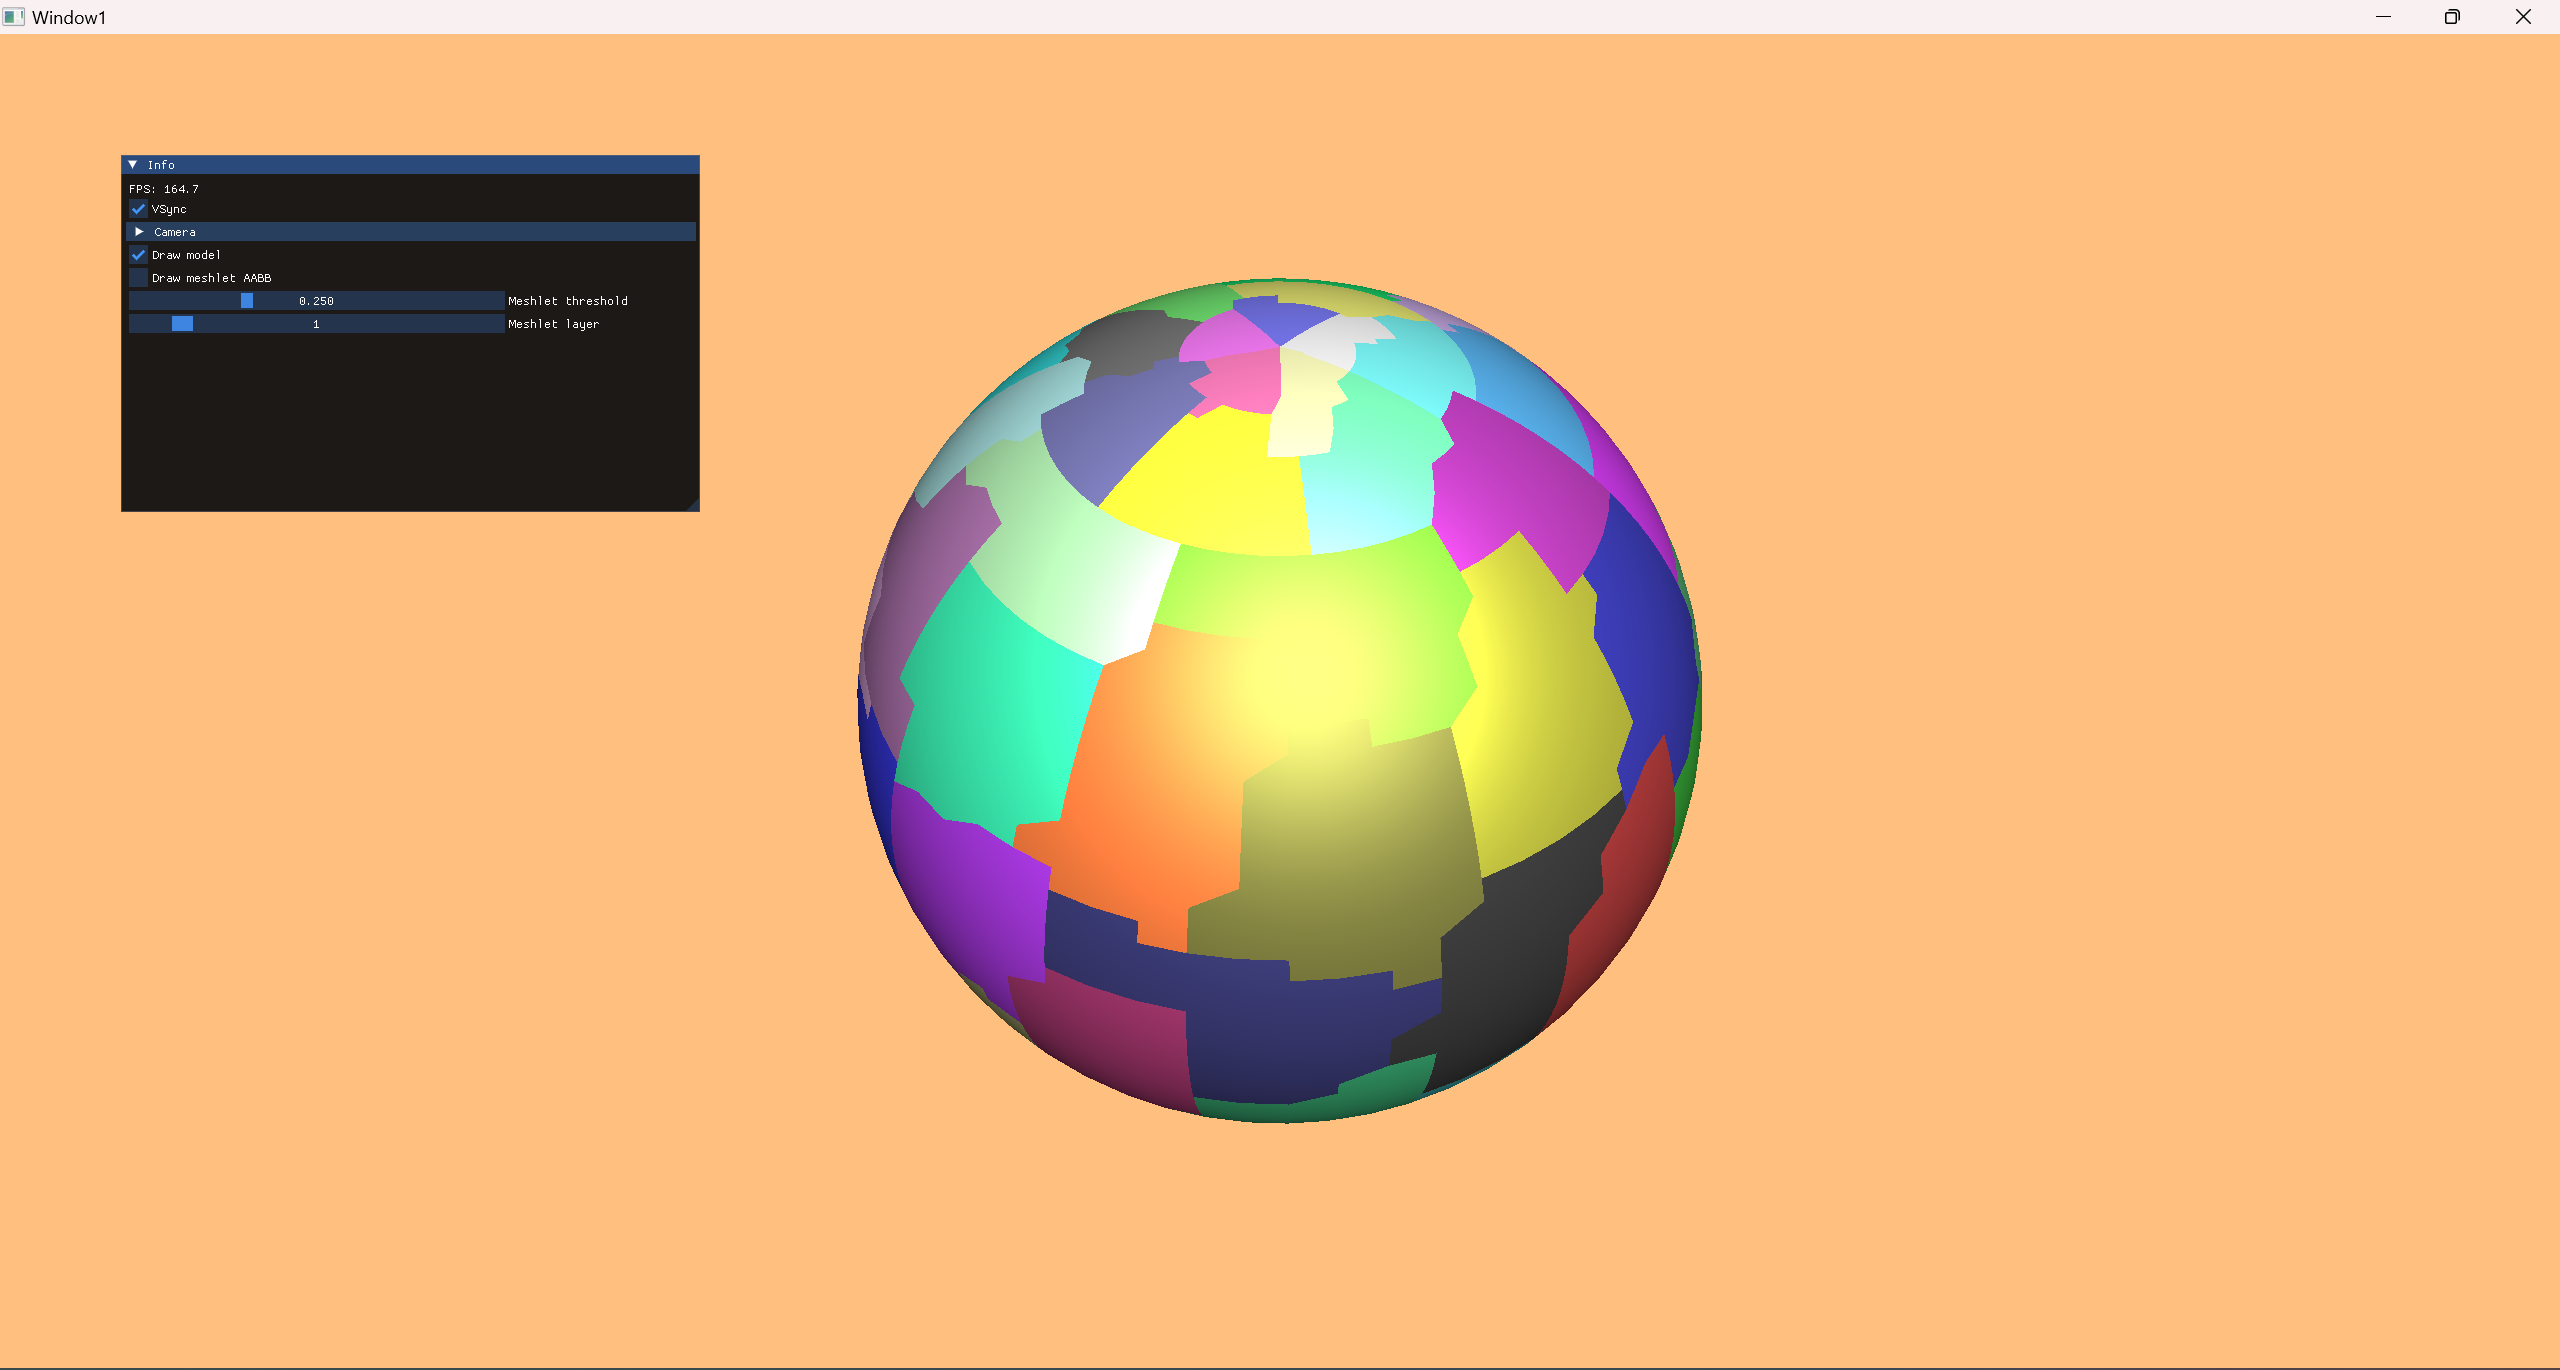
\includegraphics[width=\textwidth]{sphere0.png}
    \end{frame}

    \begin{frame}{Проблемы при реализации: последствия}
        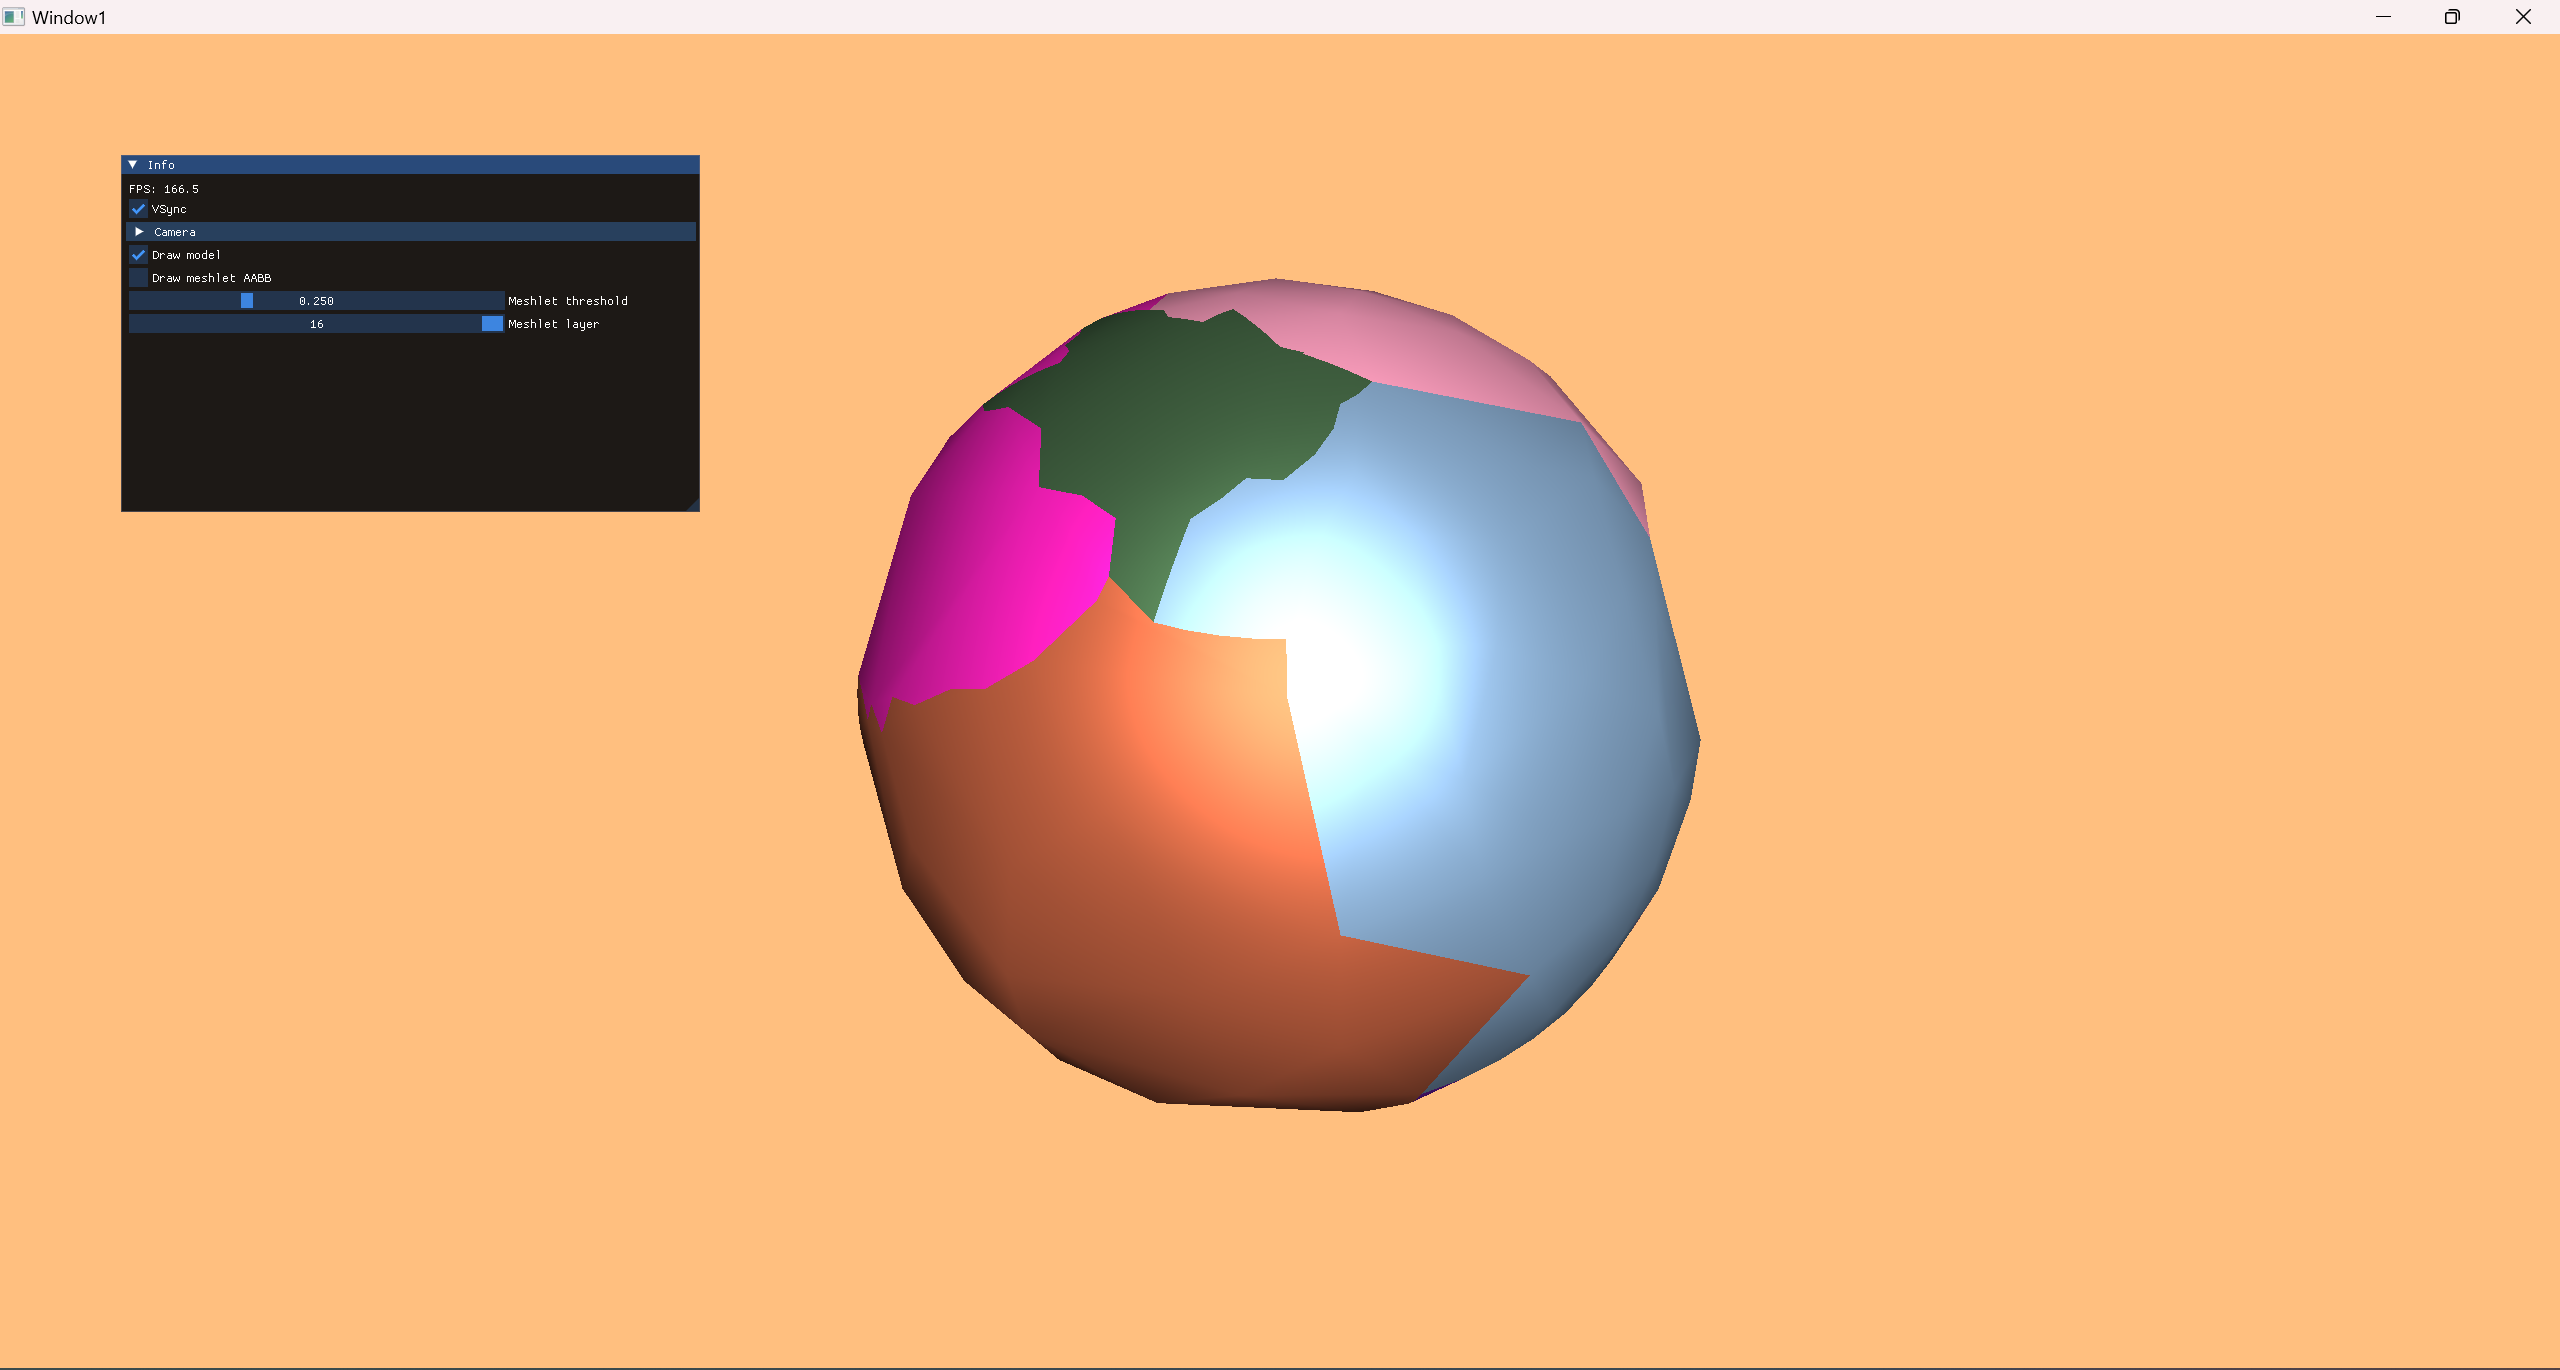
\includegraphics[width=\textwidth]{sphere1.png}
    \end{frame}

    \begin{frame}{Принципиальные ограничения}
        \begin{itemize}
            \item
            Для учёта положения камеры в оценке ошибки
            используется AABB\footnote{
                Axis Aligned Bounding Box (AABB) ---
                прямоугольный параллелепипед
                с рёбрами, параллельными осям координат,
                описывающий заданную геометрию.
            } мешлета и суммы его родителей.
            При любом движении вершин исходной модели
            относительно друг друга потребуется
            пересчёт AABB всех вершин графа,
            чтобы избежать разрывов по швам.
            Такой пересчёт займёт значительное время,
            из-за этого технология работает только со
            статичной геометрией;

            \item
            Кластеризация треугольников и последующее уменьшение
            детализации сильно завязаны на то,
            что исходная модель --- поверхность замкнутого объёма.
            Основная часть крупных объектов в компьютерных играх
            попадают под такое определение.
        \end{itemize}
    \end{frame}

    \begin{frame}{Принципиальное ограничение: поддержка}
        Mesh Shader появились сравнительно недавно,
        например, видеокарты NVidia поддерживают
        их только начиная с 20xx серии.
        Согласно статистике Steam на март 2024,
        32\% используемых игроками видеокарт NVidia
        --- более ранних серий,
        это 23\% от всех устройств.

        \bigskip

        Однако стоит разделять
        23\% от тех компьютеров,
        с которых была собрана статистика,
        и 23\% всех игроков ---
        часть игроков имеет несколько компьютеров,
        часть отказывается от сбора статистики,
        а для части игроков основная платформа
        --- игровая консоль, а не персональный компьютер.
    \end{frame}

    \begin{frame}{Принципиальное ограничение: объём}
        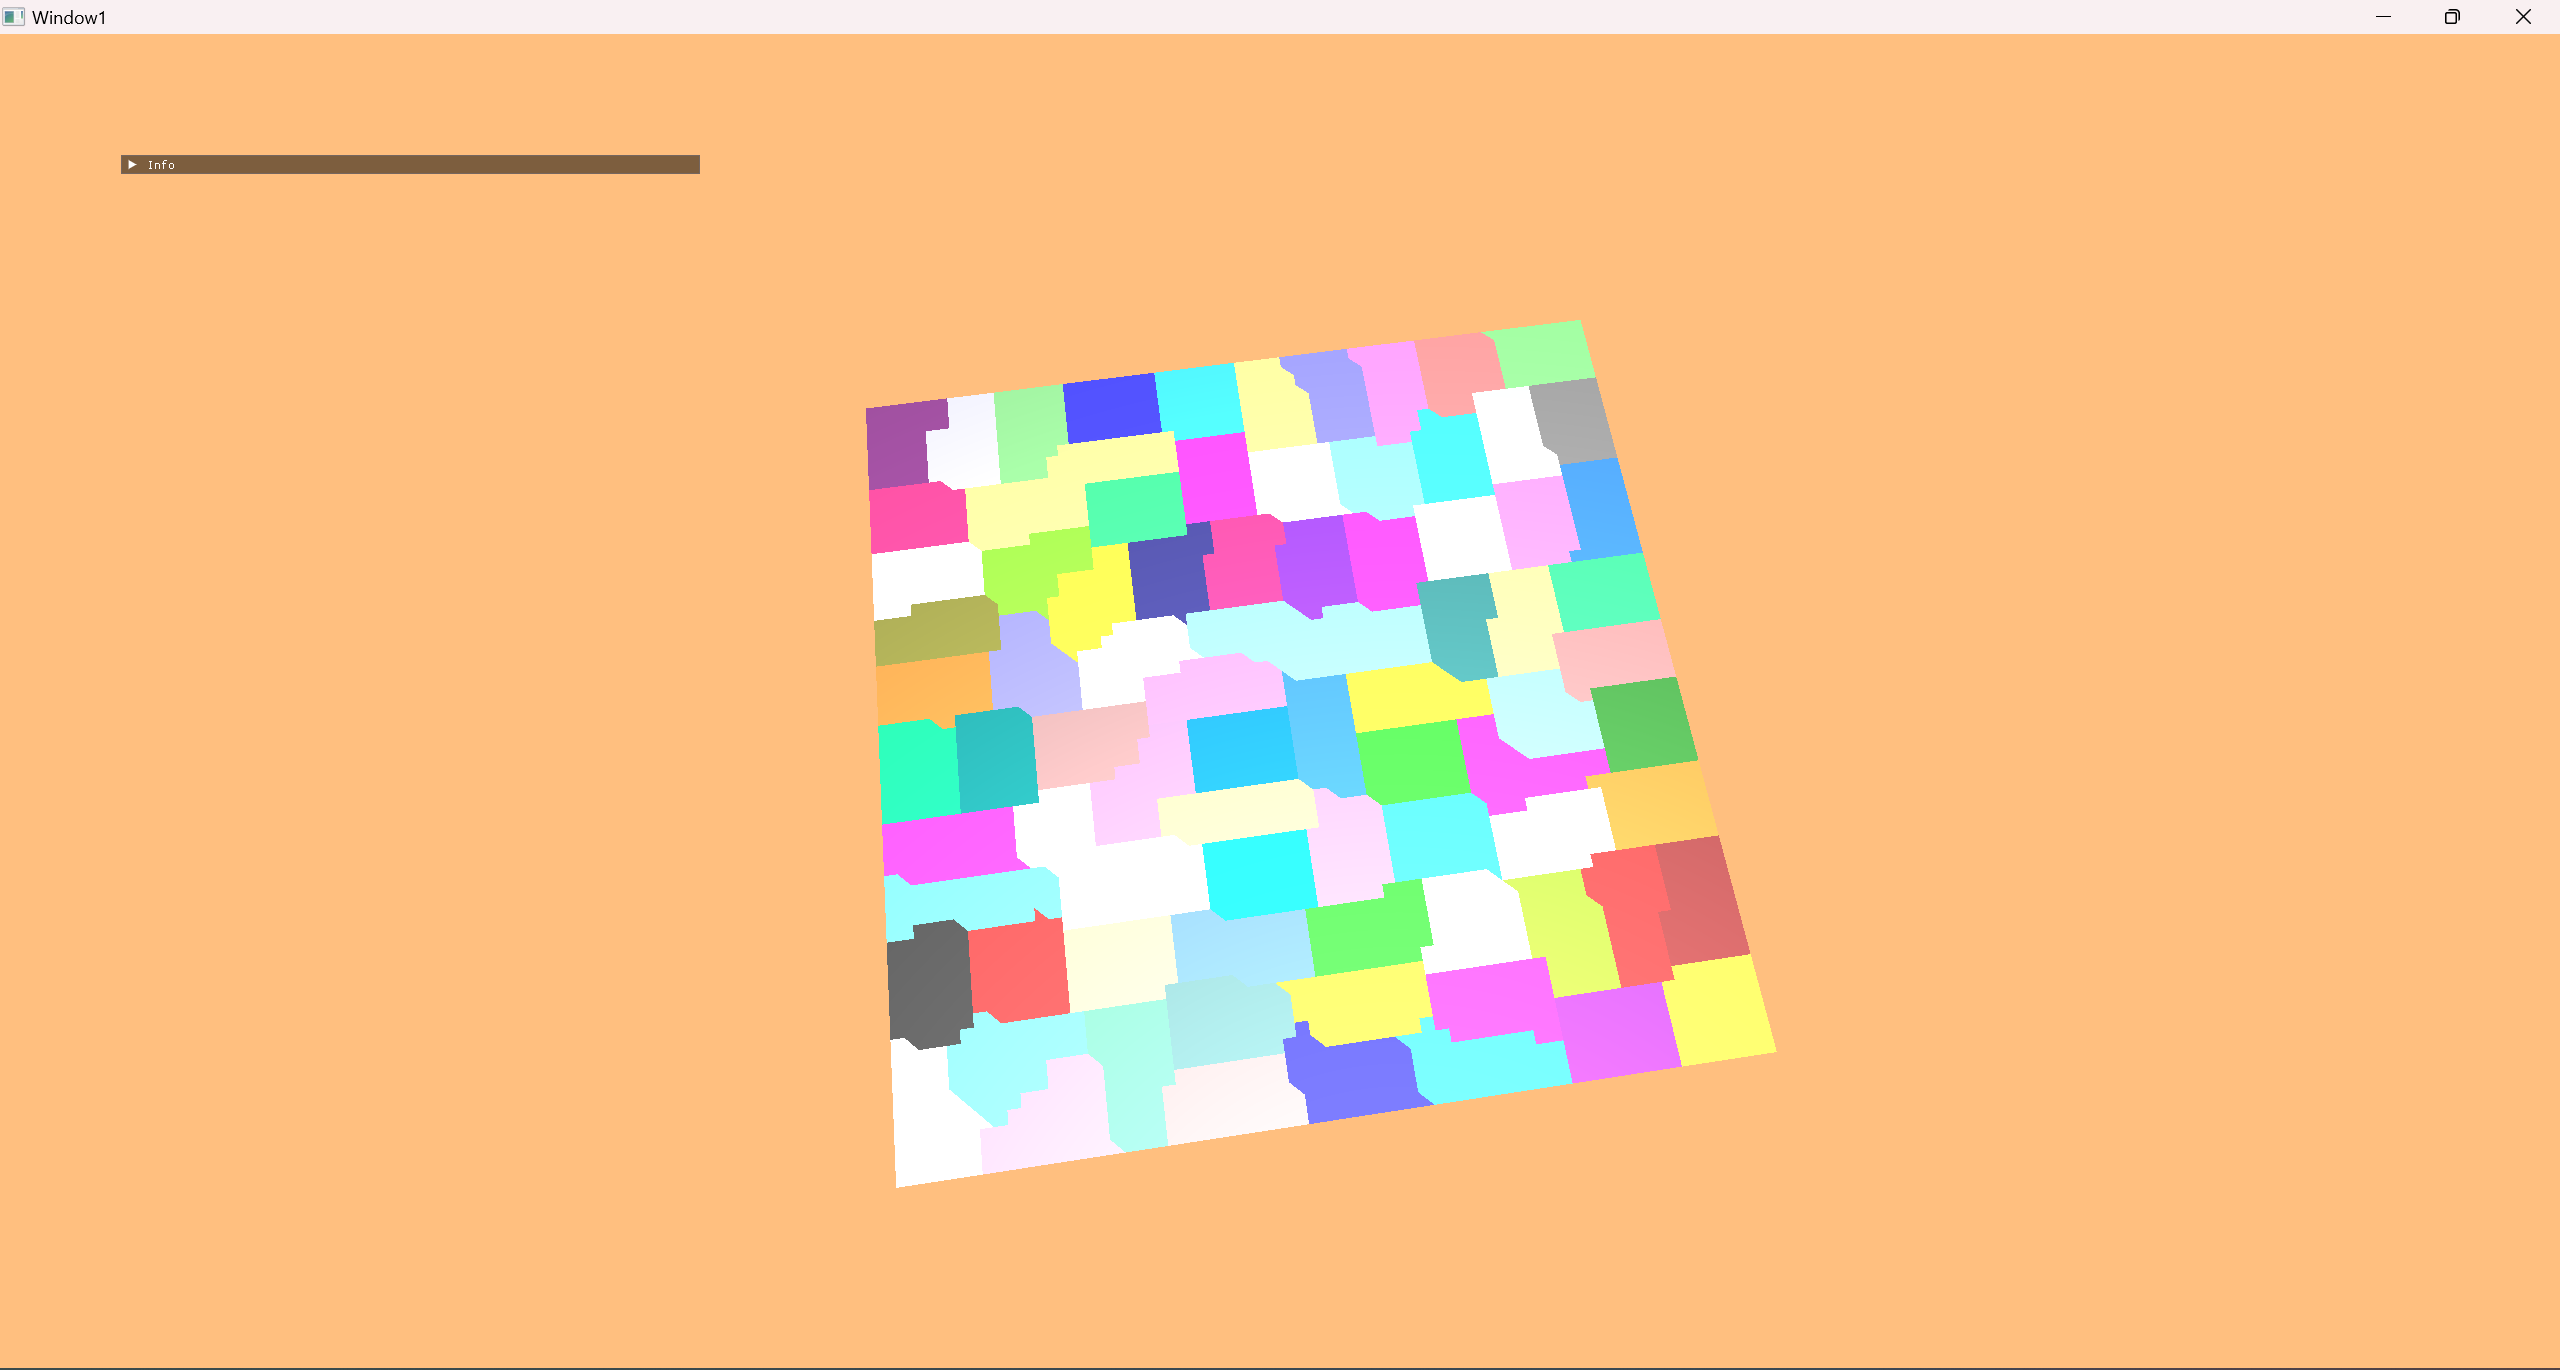
\includegraphics[width=\textwidth]{plane0.png}
    \end{frame}

    \begin{frame}{Принципиальное ограничение: объём}
        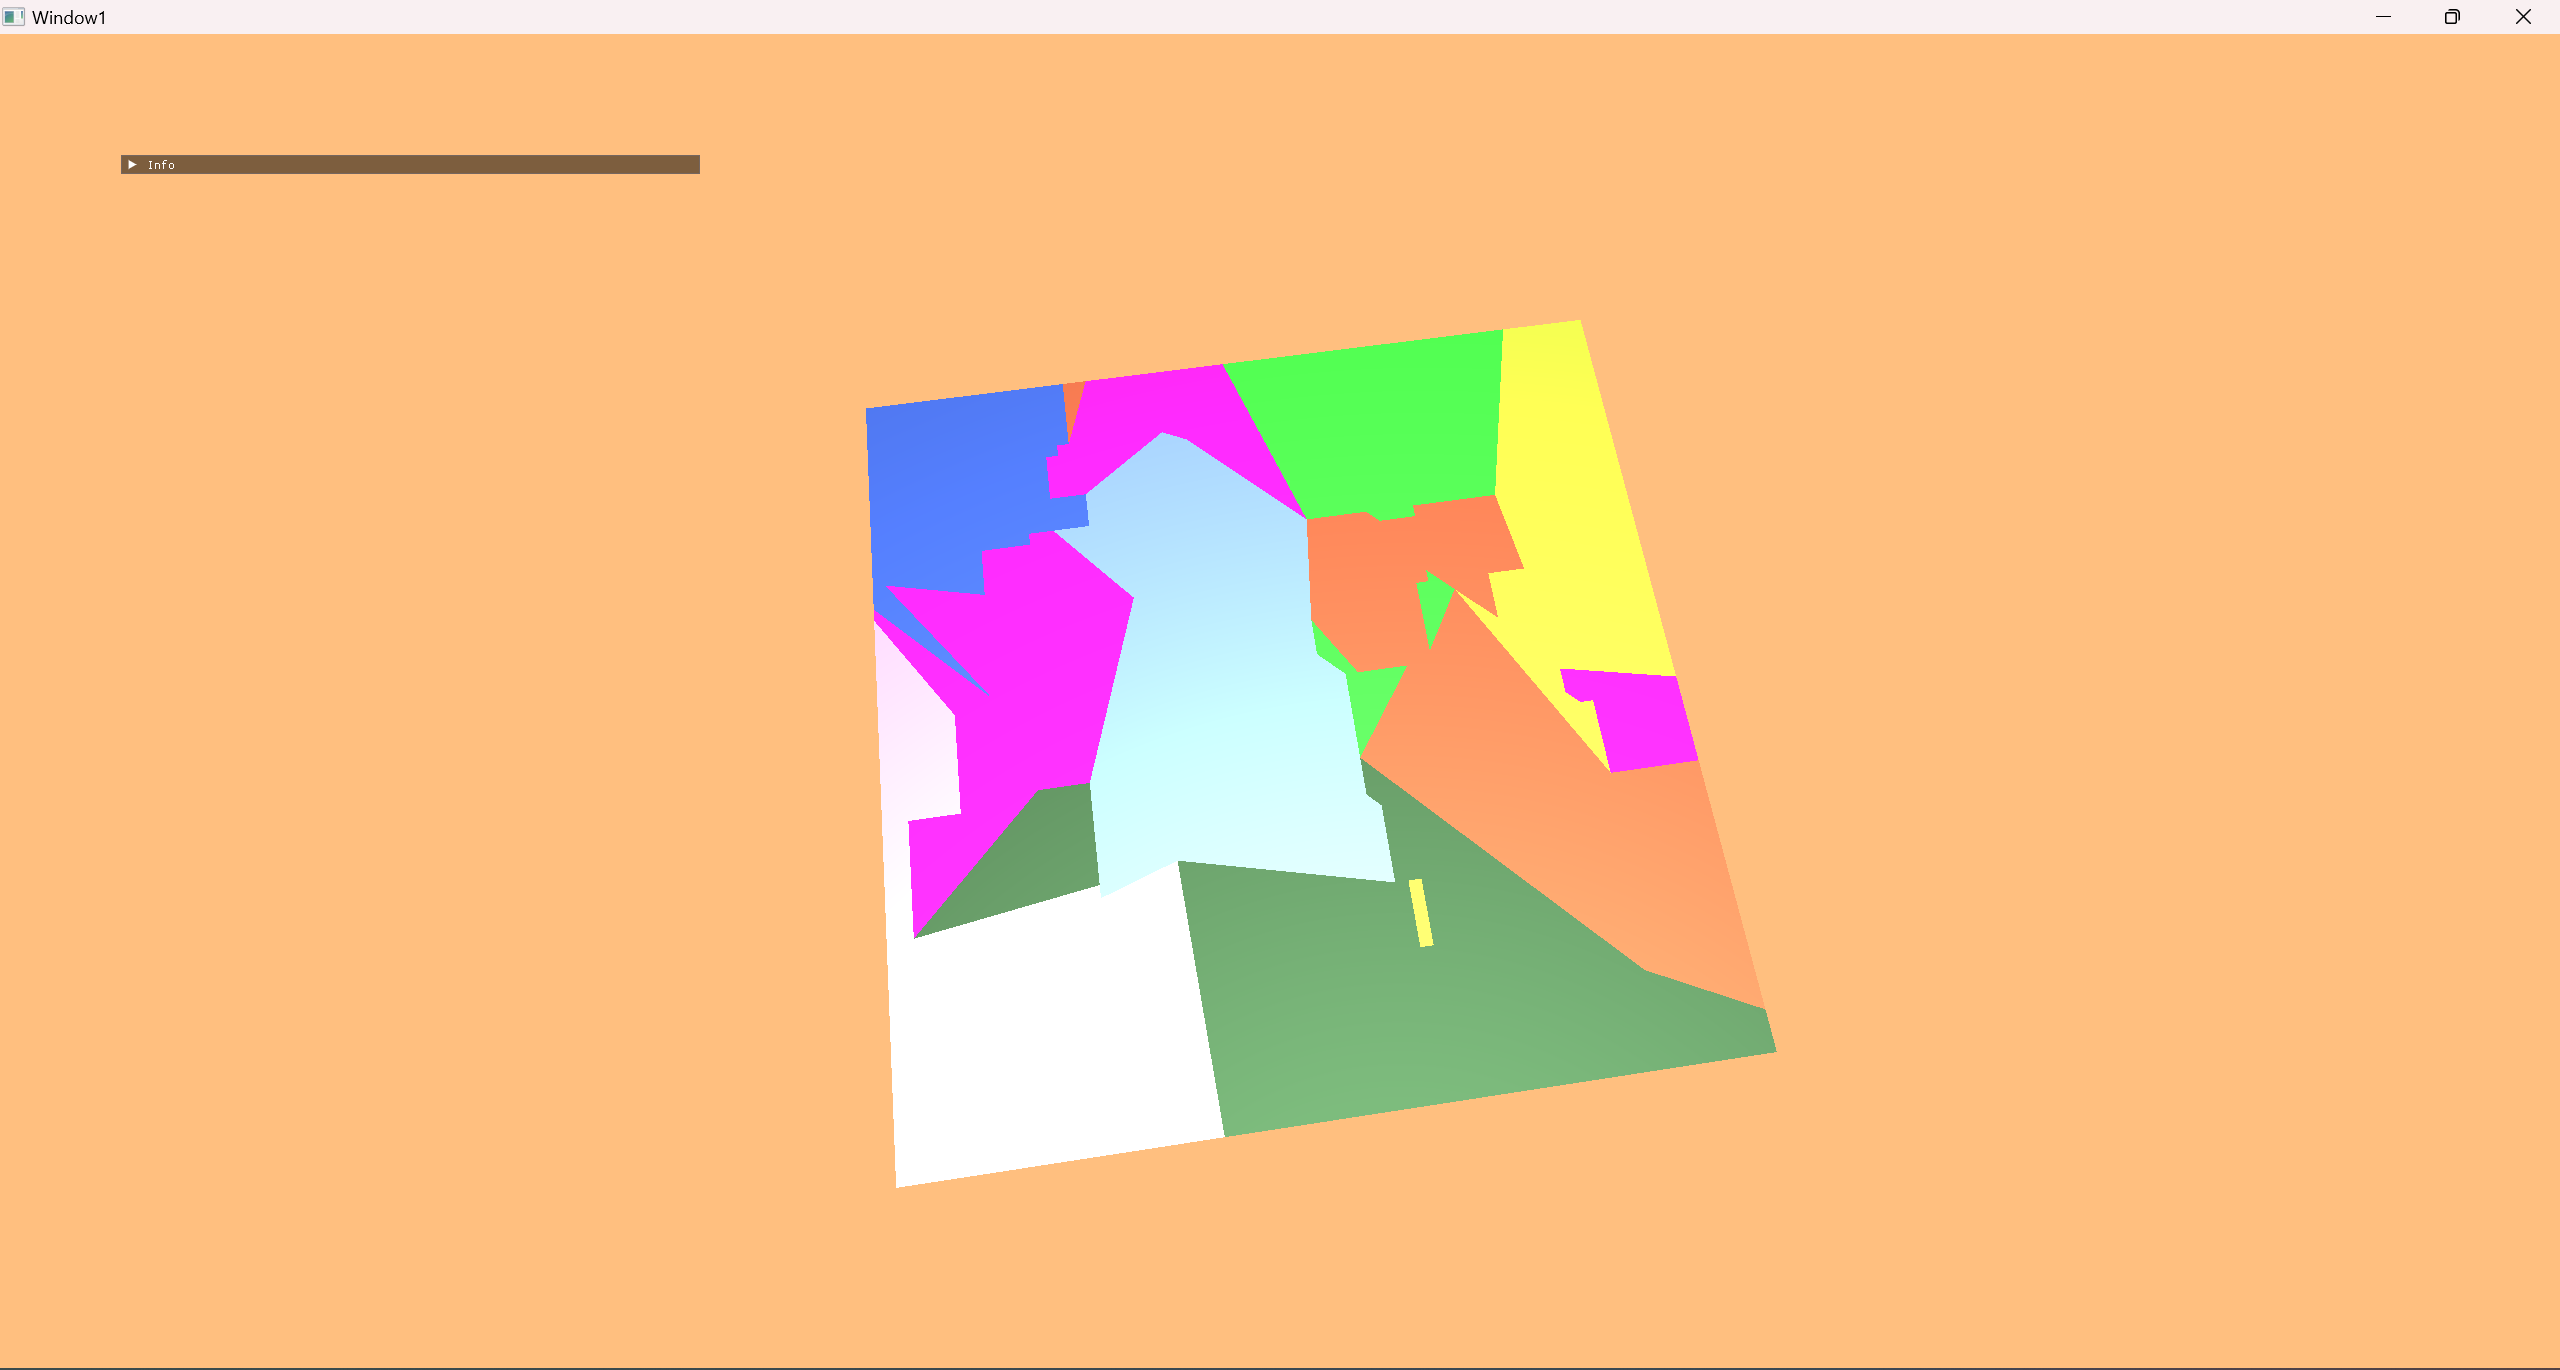
\includegraphics[width=\textwidth]{plane1.png}
    \end{frame}

    \begin{frame}{Сравнение с некластерной детализацией}
        Пока не проводилось
    \end{frame}

    \begin{frame}{Результаты}
        \begin{itemize}
            \item Выявлены существтенные проблемы,
            возникающие при реализации
            динамической кластерной детализации;

            \item Выявлены принципиальные
            ограничения технологии,
            которые существенны при принятии решения
            о реализации полной, а не упрощённой,
            версии и интеграции в существующий движок;
        \end{itemize}
    \end{frame}
\end{document}
